\documentclass[14pt, a4paper]{article}
\usepackage{fullpage}
\usepackage[top=2cm, bottom=2cm, left=2.5cm, right=2cm]{geometry}
\usepackage{amsmath,amsthm,amsfonts,amssymb,amscd}
\usepackage{fancyhdr}
\usepackage{fixltx2e}
\usepackage{mathrsfs}
\usepackage{listings}
\usepackage{color}
\usepackage{relsize}
\usepackage{graphicx}
\usepackage[utf8]{inputenc}
\usepackage[T1]{fontenc}
\usepackage[english, russian]{babel}

\definecolor{dkgreen}{rgb}{0,0.6,0}
\definecolor{gray}{rgb}{0.5,0.5,0.5}
\definecolor{mauve}{rgb}{0.58,0,0.82}

\DeclareMathSizes{14}{24}{18}{12}

\lstset{frame=tb,
  language=Python,
  aboveskip=3mm,
  belowskip=3mm,
  showstringspaces=false,
  columns=flexible,
  basicstyle={\small\ttfamily},
  numbers=none,
  numberstyle=\tiny\color{gray},
  keywordstyle=\color{blue},
  commentstyle=\color{dkgreen},
  stringstyle=\color{mauve},
  breaklines=true,
  breakatwhitespace=true,
  tabsize=3
}

\renewcommand{\thesection}{\arabic{section}.}
\renewcommand{\thesubsection}{\thesection\arabic{subsection}.}
\renewcommand{\thesubsubsection}{\thesubsection\arabic{subsubsection}.}

\title {Лабораторная работа №1 \\ Решение нелинейного уравнения методом простой итерации}
\author {Журик Никита, 6 группа}
\date {26.03.2019}


\begin{document}
\pagenumbering{gobble}
\begin{titlepage}
\begin{center}
\large{БЕЛОРУССКИЙ ГОСУДАРСТВЕННЫЙ УНИВЕРСИТЕТ 

ФАКУЛЬТЕТ ПРИКЛАДНОЙ МАТЕМАТИКИ И ИНФОРМАТИКИ

КАФЕДРА ВЫЧИСЛИТЕЛЬНОЙ МАТЕМАТИКИ}
\end{center}
\vspace*{\fill}
\begin{center}
Лабораторная работа 1

\large{\textbf{Метод простой итерации решения нелинейного уравнения.}}

Вариант 7
\end{center}
\begin{flushright}
\textbf{Выполнил:}

Журик Никита Сергеевич \\ 2 курс, 6 группа

\textbf{Преподаватель:}

Будник Анатолий Михайлович
\end{flushright}
\vspace*{\fill}
\begin{center}
Минск, 2019
\end{center}
\end{titlepage}

\tableofcontents
\newpage

\newpage
\pagenumbering{arabic}

  \section{Постановка задачи}
    \begin{enumerate}
      \item
      Отделить корень и определить отрезок $[a; b]$.
      \item
      Проверить условия теоремы о сходимости метода простой итерации.
      \item
      Решить нелинейное уравнение $f(x) = 0$ методом простой итерации с точностью $\epsilon = 10^{-8}$.
      \item
      Найти априорную и фактическую оценки количества итераций.
      \item
      Вычислить невязку решения.
      \item
      Проанализировать полученные результаты.
    \end{enumerate}
  \section{Алгоритм решения}
  \begin{itemize}
    \item
    Сперва отделим корни уравнения $f(x) = 0$ при помощи таблицы значений. Таким образом, для каждого корня получим некоторый отрезок, содержащий сам корень, причём на этом отрезке функция в левой части монотонна.
    \item
    Для решения уравнения \begin{equation}f(x) = 0\end{equation} методом простой итерации необходимо представить его в каноническом виде: \begin{equation}x = \phi(x)\end{equation}
    После чего построим итерационный процесс \begin{equation}x^{k + 1} = \phi(x^k); k = 0, 1, 2, ...; x^0\end{equation}
    Условием остановки послужит выполнение следующего условия: \begin{equation}|x^{k + 1} - x^k| \leq \epsilon,\end{equation} где $\epsilon$ - некоторое заданное число (требуемая точность).\\
    При выполнении условий теоремы о сходимости метода простой итерации данный итерационный процесс будет сходиться к единственному корню на отрезке отделения корня.
    \item
    \textbf{Теорема о сходимости метода простой итерации:}\\
    Если выполняются следующие условия:
      \begin{enumerate}
        \item
          Функция $\phi(x)$ определена и непрерывна на отрезке отделения корня $|x - x^*| \leq \delta$, а также удовлетворяет условию Липшица с константой меньше 1,
          то есть является сжимающим отображением: \begin{equation}|\phi(x) - \phi(\tilde{x})| \leq q|x - \tilde{x}|,\end{equation}
          где $0 < q < 1$ - константа Липшица;
        \item
          Для начального приближения $x^0$ верно неравенство $|x^0 - \phi(x^0)| \leq m$;
        \item
          Для $m$, $q$ и $\delta$ справедливо неравенство \begin{equation}\frac{m}{1 - q} \leq \delta,\end{equation}
      \end{enumerate} то:
      \begin{enumerate}
        \item
        Уравнение $(1)$ имеет корень на рассматриваемом отрезке;
        \item
        Итерационная последовательность $(2)$ сходится, причём к корню уравнения $(1)$;
        \item
        Скорость сходимости метода простой итерации оценивается неравенством \begin{equation}|x^* - x^k| \leq \frac{m}{1 - q}q^k\end{equation}
      \end{enumerate}
      Из теоремы следует априорная оценка количества итераций: \begin{equation}k \geq \frac{ln(\frac{\epsilon(1-q)}{m})}{ln(q)}\end{equation}
  \end{itemize}
  \section*{Решение конкретного уравнения}
  \begin{itemize}
    \item
    Рассмотрим уравнение $3ln^2x + 6lnx - 5 = 0$. Приведём его к каноническому виду: \begin{equation}x = e^{\frac{-3ln^2x + 5}{6}}\end{equation}
    \item
    Тогда итерационный процесс будет выглядеть следующим образом: \begin{equation}x^{k + 1} = e^{\frac{-3ln^2x^k + 5}{6}}; k = 0, 1, 2, ...; x^0\end{equation}
    \item
    Отделим корни. Исходное уравнение имеет два корня (см. рис. 1). Для их отделения построим таблицу значений функции: разобьём отрезок $[0.01; 3]$ на 20 равных частей и вычислим значения
    на концах полученных отрезков и найдём те отрезки, на которых функция меняет знак. Таким образом, получим отрезки $[0.01; 0.167...]$ и $[1.741...; 1.898...]$.
    \begin{figure}[h!]
    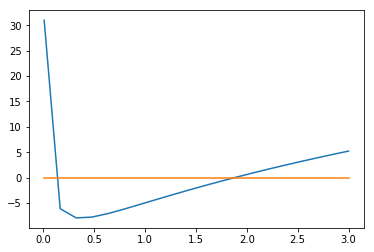
\includegraphics[width=300pt]{f(x).png}
    \caption{$f(x)$}
    \end{figure}
    \item
    Проверим условия теоремы о сходимости метода простой итерации.
    \begin{enumerate}
    \item
    Рассмотрим отрезок, содержащий меньший корень. Вывод программы содержит всю необходимую информацию для проверки теоремы:
\begin{align*}
Lipschitz\ hypothesis\ not\ satisfied\ with\ q &= 2.9585368758514967\\
max|\phi'(x)| &= 4.973182732158916\\
m &= 0.19802324885811545\\
q &= 2.9585368758514967\\
\delta &= 0.14950000000000002\\
\frac{m}{1 - q} &= 0.10110774594020475\\
\frac{m}{1 - q} &\leq \delta
\end{align*}
    Нетрудно видеть, что выполняются все условия теоремы кроме условия Липшица, а значит, построенная итерационная последовательность не обязательно сойдётся.

    \item
    Теперь рассмотрим больший корень:
\begin{align*}
Lipschitz\ hypothesis\ satisfied\ with\ q &= 0.6320492947765582\\
max|\phi'(x)| &= 0.6332465196036281\\
m &= 0.00036110825724988693\\
q &= 0.6320492947765582\\
\delta &= 0.14950000000000002\\
\frac{m}{1 - q} &= 0.0009814039003692094\\
\frac{m}{1 - q} &\leq \delta
\end{align*}
    На отрезке, содержащем второй корень, выполнены все условия теоремы, а значит, на этом отрезке итерационная последовательность обязана сойтись к корню.
    Оценим количество итераций: \begin{equation}\frac{ln(\frac{\epsilon(1-q)}{m})}{ln(q)} = 25.0533\end{equation}
    Тогда \begin{equation}k_{aprior} = 26\end{equation}

    \end{enumerate}
  \end{itemize}
  \section{Листинг программы}
  Для реализации алгоритма был использован Python и библиотеки numpy и matplotlib.

\begin{lstlisting}

#Common.py

#!/usr/bin/env python
# coding: utf-8

#Plot the function

import math
import numpy as np
import matplotlib.pyplot as plt

samples = 20
left_border = 0.01
right_border = 3
delta = (right_border - left_border) / samples
eps = 10 ** -5

def f(x):
    l = math.log(x)
    return 3 * l ** 2 + 6 * l - 5

def f_prime(x):
    l = math.log(x)
    return 6 * (l + 1) / x

def phi(x):
    return math.e ** ((-3 * math.log(x) ** 2 + 5) / 6)

def phi_prime(x):
    return -phi(x) * math.log(x) / x

x_values = np.linspace(left_border, right_border, samples)
f_values = np.zeros(np.shape(x_values))

for i in range(samples):
    f_values[i] = f(x_values[i])

#Root separation

def separate_roots(x_values, f_values):
    intervals = [ ]
    for i in range(samples - 1):
        if (f_values[i + 1] * f_values[i] < 0):
            intervals = np.append(intervals, i)
    return intervals

intervals = separate_roots(x_values, f_values)
        
print(intervals)

#SimpleIteration.py

#!/usr/bin/env python
# coding: utf-8

from Common import *

plt.plot(x_values, f_values)
plt.plot(x_values, np.zeros(np.shape(x_values)))
plt.show()

#Check all conditions

def check_Lipschitz(interval):
    x = x_values[interval]
    xwave = x_values[interval + 1]
    q = 15
    temp_q = 0
    q_samples = 10000
    for i in range(q_samples):
        diff = (i + 1) * (xwave - x) / (2 * (q_samples))
        left = (x + xwave) / 2 - diff
        right = left + 2 * diff
        temp_q = abs((phi(right) - phi(left)) / (right - left))
        #print("Calculating q on interval [{0}; {1}]; q_{2} = {3}".format(left, right, i, temp_q))
        if (temp_q < q):
            q = temp_q
            
    if (q < 1):
        print("Lipschitz hypothesis satisfied with q =", q)
    else:
        print("Lipschitz hypothesis not satisfied with q =", q)
    return q
        
def check_phi_prime(interval):
    x = x_values[interval]
    xwave = x_values[interval + 1]
    max_phi_prime = 0
    cur_phi_prime = 0
    for cur_x in np.linspace(x, xwave, 300):
        cur_phi_prime = abs(phi_prime(cur_x))
        if (cur_phi_prime > max_phi_prime):
            max_phi_prime = cur_phi_prime
    print("max|phi'(x)| =", max_phi_prime)
    return max_phi_prime

#Solve the equation using simple iteration method

def find_root(interval):
    x_left = x_values[interval]
    x_right = x_values[interval + 1]
    lam = f(x_left) / f(x_right)
    old_x = (x_left - lam * x_right) / (1 - lam)
    #old_x = (x_left + x_right) / 2
    new_x = phi(old_x)
    m = abs(new_x - old_x)
    print("x[0] =", old_x, "; x[1] =", new_x)
    num_iter = 1

    while (abs(new_x - old_x) >= eps):
        old_x = new_x
        new_x = phi(old_x)
        num_iter = num_iter + 1

    print("X* =", new_x, "; f(X*) =", f(new_x))
    print("|x^(k+1) - x^k| =", abs(new_x - old_x))
    print("Number of iterations:", num_iter)
    return m

for i in intervals:
    interval = int(i)
    print("Interval #", interval + 1)
    print("Interval borders:", x_values[interval], x_values[interval + 1])
    m = find_root(interval)
    print()
    q = check_Lipschitz(interval)
    max_prime = check_phi_prime(interval)
    print()
    print("m =", m)
    print("q =", q)
    print("delta =", delta)
    print()
    print("m / (1 - q) =", abs(m / (1 - q)))
    if abs(m / (1 - q)) <= delta:
        print("m / (1 - q) <= delta")
    else:
        print("m / (1 - q) > delta")
    print()

\end{lstlisting}

  \section{Вывод программы}
\begin{verbatim}
Interval # 1
Interval borders: 0.01 0.1673684210526316
x[0] = 0.14134905726406316 ; x[1] = 0.3393723061221786
X* = 1.8832389946260963 ; f(X*) = 1.9901603920402522e-08
|x^(k+1) - x^k| = 9.868320605121994e-09
Number of iterations: 43

Lipschitz hypothesis not satisfied with q = 2.9585368758514967
max|phi'(x)| = 4.973182732158916

m = 0.19802324885811545
q = 2.9585368758514967
delta = 0.14950000000000002

m / (1 - q) = 0.10110774594020475
m / (1 - q) <= delta

Interval # 12
Interval borders: 1.7410526315789476 1.8984210526315792
x[0] = 1.8834601238122997 ; x[1] = 1.8830990155550498
X* = 1.8832389945872872 ; f(X*) = 1.9699690767538414e-08
|x^(k+1) - x^k| = 9.768200470716693e-09
Number of iterations: 24

Lipschitz hypothesis satisfied with q = 0.6320492947765582
max|phi'(x)| = 0.6332465196036281

m = 0.00036110825724988693
q = 0.6320492947765582
delta = 0.14950000000000002

m / (1 - q) = 0.0009814039003692094
m / (1 - q) <= delta
\end{verbatim}

  \section{Выводы}
  \begin{itemize}
  \item
  Из результатов выполнения программы можно видеть, что метод простой итерации действительно не сошёлся в окрестности меньшего корня, а вместо этого сошёлся к большему корню. Это связано со свойствами функции $\phi(x)$ в окрестности левого корня.
  На соответствующем отрезке эта функция не является сжимающим отображением, а значит, условие теоремы не было выполнено.
  \item
  В окрестности большего корня метод простой итерации сошёлся к корню с требуемой точностью, однако условие остановки оказалось не достоверным: невязка равна $f(X^*) = 1.9699690767538414e-08$, что больше требуемой точности $\epsilon = 10^{-8}$,
  несмотря на то, что $|x^{k+1} - x^k| = 9.768200470716693e-09$.
  \item
  Также стоит отметить, что априорная оценка количества итераций для второго корня оказалась довольно точной: $26$ итераций, когда реальное число итераций равно $24$. 
  \end{itemize}

\end{document}